%% Submissions for peer-review must enable line-numbering 
%% using the lineno option in the \documentclass command.
\documentclass[fleqn,10pt,lineno]{wlpeerj}
\usepackage{algorithm}
\usepackage{algpseudocode}

\title{A Cluster-Conditioned Explainable AI Framework for Interpretable Decision Support: Surrogate Rule Extraction for Agricultural Training Allocation}

\author[1]{Kitti Chiewchan}
\author[2]{Jumtip Seneerattanaprayul}
\affil[1]{Computer Education Program, Faculty of Education, Bansomdejchaopraya Rajabhat University, Bangkok, Thailand}
\affil[2]{Department of Agricultural and Resource Economics, Faculty of Economics, Kasetsart University, Bangkok, Thailand}
\corrauthor[1]{Kitti Chiewchan}{kitti.ch@bsru.ac.th}

\begin{abstract}
Allocating training programs to farmers with diverse backgrounds requires transparent methods that explain which personal characteristics drive better learning outcomes. We propose SAR (Segment--Attribute--Recommend), a systems architecture designed for targeted resource allocation. The SAR framework operates in three sequential stages: (1) grouping individuals into homogeneous segments based on their profiles, (2) identifying key feature attributions within each segment, and (3) translating these analytical findings into simple, operational IF--THEN decision rules.

We validated the SAR framework using agricultural training data from $n=833$ participants in Thailand's Smart Farmer program. The system identified three distinct segments, each driven by different factors for skill improvement: baseline experience, production management capability, and educational background. The extracted decision rules achieved an accuracy of 91.4\% on held-out test data, 95.3\% $\pm$ 2.5\% under cross-validation, and 93.3\% across the full dataset.

Our framework provides a transparent, auditable tool for resource allocation in agricultural extension and broader policy planning. Unlike standard black-box models, SAR generates human-readable rules that non-technical administrators can deploy directly without machine learning expertise.
\end{abstract}

\begin{document}

\flushbottom
\maketitle
\thispagestyle{empty}

\section*{Introduction}
Providing agricultural training that meets the specific needs of individual farmers remains a critical challenge. Most national programs still rely on a uniform curriculum for all participants, regardless of their prior skill levels or economic backgrounds. This rigid approach often leads to inefficient resource allocation and poor adoption rates, as many farmers find the material either too basic or too advanced. To improve policy outcomes, extension services need a systematic method to match training resources with a farmer's specific skills, risk attitudes, and capacities.

While machine learning models can accurately predict training success, implementing them in public policy requires operational transparency. Administrators and policymakers must be able to justify resource allocation decisions, making opaque black-box models unsuitable for public sector deployment. Effective intervention requires knowing not just which outcomes are likely to occur, but exactly why specific student profiles respond differently to training.

Explainable AI (XAI) methods, particularly SHAP (SHapley Additive exPlanations), offer a way to identify the underlying drivers behind model predictions. However, existing XAI applications in agriculture suffer from two main limitations. First, most studies focus on generating complex diagnostic charts rather than translating model insights into actionable field guidelines. Second, global explanation models treat the target population as a single homogeneous group, thereby overlooking how different types of farmers respond to training interventions.

To address these limitations, this study introduces SAR (Segment--Attribute--Recommend), a three-stage decision support framework. The system clusters the target population into distinct segments, identifies key drivers within each sub-population, and extracts transparent IF--THEN rules using a global surrogate tree. Our approach enables non-technical personnel to implement data-driven recommendations directly in the field without needing active machine learning systems or programming skills.

\subsection*{Study Contribution}
This study provides three key contributions to the field of interpretable machine learning in agriculture:
\begin{enumerate}
    \item \textbf{Cluster-Conditioned XAI Framework:} We move beyond global feature importance models by accounting for population heterogeneity. Instead of generating a single ranking for all observations, we perform feature attribution within locally homogeneous subgroups, capturing distinct training drivers across different farmer segments.
    \item \textbf{Structured Surrogate Rule Extraction:} We present a clear pipeline to bridge the gap between model interpretation and fieldwork. By mapping SHAP values into compact decision trees, we turn SHAP findings into simple IF--THEN rules that field staff can use straight away.
    \item \textbf{Generalizable Decision Support Architecture:} We deliver a reproducible, modular pipeline that separates population segmentation, attribution analysis, and rule generation. This pipeline can also be used in other public programs where 
people have different needs and decisions must be easy to explain.
\end{enumerate}

%%─────────────────────────────────────────────────────────────────────────────
\section{Literature Review}
%%─────────────────────────────────────────────────────────────────────────────

\subsection{Machine Learning in Agriculture}
Machine learning and computer vision are now foundational technologies in modern agriculture, driving developments in crop monitoring, soil analysis, and livestock management \citep{liakos2018}. While deep learning models such as CNNs excel at complex pattern recognition tasks like cattle identification \citep{hossain2022cattle}, recent research has focused significantly on improving deployment efficiency. For example, advances in TinyML now allow optimized deep architectures to run real-time acoustic pest detection directly on low-cost microcontrollers \citep{kazeneza2026}. Similarly, hybrid predictive frameworks have optimized multi-source data processing for soil nutrient management \citep{ennaji2023nutrient} and agricultural price forecasting \citep{zhao2026}. These trends show that agricultural AI is moving away from generic models toward specialized, resource-efficient systems tailored to specific operational constraints \citep{kamilaris2018}.

\subsection{Decision Support Systems (DSS) and Integration}
Moving from automated prediction to effective field deployment requires integrating data streams, predictive models, and management processes into a unified system \citep{liu2009}. Isolated, standalone predictive models often fail to capture the dynamic constraints of real-world environments, highlighting the need for Integrated Decision Support Systems (IDSS) that offer coordinated planning capabilities \citep{liu2009}. Comparative studies in resource management show that advanced DSS platforms are frequently underutilized if they ignore user constraints, data availability, or stakeholder feedback \citep{volk2010}. Consequently, effective systems must serve as accessible learning platforms that present clear choices, bridging the gap between technical algorithms and the daily needs of field personnel \citep{volk2010}.

\subsection{Explainable AI (XAI) for Decision Support}
As predictive architectures grow more complex, their black-box nature limits the trust and regulatory compliance needed for public administration \citep{hassija2024}. Current XAI literature emphasizes organizing explainability methods into clear structural taxonomies—such as feature-based, example-based, or neural-symbolic approaches—to help developers align explanation outputs with specific stakeholder needs \citep{speith2022, dwivedi2023}. Model-agnostic feature attribution methods, particularly SHAP, are widely valued because their solid mathematical foundations ensure stable local and global explanations across diverse model families \citep{lundberg2017, lundberg2020, yu2026, guidotti2019}. However, while XAI has been used for agricultural risk and yield modeling \citep{ghosal2018, ryo2022}, research rarely converts these diagnostic findings into operational rules. This study addresses this gap by converting raw feature attributions into actionable rule structures for field deployment.

\subsection{Large Language Models and Agentic Systems}
Large Language Models (LLMs) have evolved beyond basic language generation toward autonomous agentic architectures capable of multi-step reasoning and environmental interaction \citep{minaee2025}. Modern frameworks organize the LLM lifecycle across pre-training, post-training alignment, and task utilization stages, giving rise to emergent reasoning capabilities \citep{zhao2026llm}. By combining structured memory modules, planning pipelines, and external tool integration, these models can execute complex workflows across scientific and engineering fields \citep{wang2024, li2025llm}. However, most current agricultural language models remain conceptual and lack validation with actual field data. Our work addresses this limitation by developing an empirical framework based on field data, providing predictable and auditable decision rules that can guide human-led extension systems.

\subsection{Farmer Heterogeneity and Training}
Target populations in agricultural sectors vary greatly regarding asset ownership, educational backgrounds, and risk management preferences, meaning uniform training structures are rarely effective \citep{feder1985, anderson2004}. Empirical evidence confirms that participants with stronger baseline skills gain more from advanced curricula, while less experienced individuals require foundational support \citep{davis2012}. Despite these differences, many public extension systems still deliver unsegmented training programs because they lack simple tools to classify their audience \citep{anderson2004}. The SAR framework addresses this operational gap by using unsupervised learning to segment populations and match individuals with appropriate training resources.

%%─────────────────────────────────────────────────────────────────────────────
\section{Methodology}
%%─────────────────────────────────────────────────────────────────────────────

\subsection{Data and Study Context}
The data for this study come from a panel survey of farmers in Thailand's Smart Farmer program, collected between 2018 and 2020. The program measures five skill areas: production management, input management, technology adoption, analysis and planning, and marketing. Farmers were assessed before and after training using a validated 5-point scale. Our main outcome variable, $Ch\_Skill$, is the difference between post-training and pre-training scores.

Missing values were rare (under 5\%). For binary and asset variables, missing values were replaced with zero, as the absence of an asset is meaningful information. For continuous skill variables, missing values were replaced with the column mean, which is appropriate given their symmetric distributions. All numeric variables were then standardized to have a mean of zero and a standard deviation of one. 

\textit{Ethics and data access:} This study followed the research protocols of the Department of Agricultural Extension, Thailand. All records were anonymized before analysis, and no personal information was used. Further details are provided in the supplementary materials.

\subsection{Farmer Segmentation}

We applied K-Means clustering \citep{macqueen1967} to 15 baseline variables, including demographics, skills, and risk perceptions.

To determine the optimal number of clusters, we evaluated four standard criteria: the Elbow method, Silhouette score, Calinski--Harabasz (CH), and Davies--Bouldin (DB) index \citep{rouseeuw1987}. As shown in Fig.~\ref{fig:elbow}, the Elbow curve shows a clear bend at $k = 3$. The other indices also support this choice, although the Silhouette score is relatively modest, which is common in Likert-scale survey data.

We further checked the robustness of this result in two ways. First, we tested values of $k$ from 2 to 5 and found that the segment structure remained stable (Fig.~\ref{fig:sensitivity}). Second, we compared K-Means with a Gaussian Mixture Model (GMM). While both methods showed moderate agreement (ARI $= 0.28$), K-Means produced more balanced and easier-to-interpret groups (Fig.~\ref{fig:gmm}).

Selecting $k = 3$ also aligns with the three-tier farmer classification used in Thailand, making the results practical for policy use.

\subsection{Predictive Modelling}
We used a Random Forest regression model \citep{breiman2001} to predict skill change ($Ch\_Skill$). Given that each farmer appears twice in the dataset (pre- and post-training), we implemented 5-fold GroupKFold cross-validation, grouping by farmer ID. This prevents data leakage by ensuring the model is never tested on a farmer it has already seen during training. We also trained an XGBoost model \citep{chen2016} as a robustness check.

We optimized the Random Forest hyperparameters via grid search. Table~\ref{tab:hyperparameters} details the search space and the final selected settings.

\begin{table}[htbp]
\centering
\caption{Random Forest hyperparameter optimization.}
\label{tab:hyperparameters}
\begin{tabular}{@{}ll@{}}
\toprule
\textbf{Parameter} & \textbf{Final Setting} \\
\midrule
Number of estimators (\texttt{n\_estimators}) & 500 \\
Min. samples per leaf (\texttt{min\_samples\_leaf}) & 10 \\
Max. features per split (\texttt{max\_features}) & \texttt{sqrt} \\
Max. tree depth (\texttt{max\_depth}) & None \\
\bottomrule
\end{tabular}
\end{table} 

\subsection{Explainable AI Analysis}
We used TreeExplainer \citep{lundberg2017} to calculate SHAP values. Overall feature importance was measured as the average absolute SHAP value across all farmers. We then repeated this analysis separately for each farmer segment to identify which variables mattered most for each group. Finally, we compared the feature rankings of our Random Forest and XGBoost models using Spearman rank correlation to ensure our findings were not dependent on the model choice.

\subsection{Decision Support Framework}

SAR operates in three stages, as shown in Fig.~\ref{fig:framework}. First, 
the \textit{Segment} stage uses K-Means to group farmers. Second, 
the \textit{Attribute} stage calculates SHAP values within each 
group. Third, the \textit{Recommend} stage uses these results to 
extract simple IF--THEN rules via a decision tree.

%%─────────────────────────────────────────────────────────────────────────────
\section{Results}
%%─────────────────────────────────────────────────────────────────────────────

Figures~\ref{fig:elbow}--\ref{fig:gmm} present the clustering validation and robustness checks. 
Figures~\ref{fig:importance}--\ref{fig:clusterShap} summarise the SHAP-based attribution analysis, 
while Fig.~\ref{fig:rules} shows the extracted decision rules.

\subsection{Farmer Segmentation}

K-Means clustering with $k=3$ identified three distinct groups of farmers (Fig.~\ref{fig:clusters}). The quality of this grouping is supported by the validation metrics (Silhouette $= 0.185$, CH $= 202.67$, DB $= 1.835$). The stability across different values of $k$ is also reflected in Fig.~\ref{fig:sensitivity}, and the comparison with GMM (Fig.~\ref{fig:gmm}) further supports the interpretability of the chosen clustering approach. Table~\ref{tab:cluster_profile} summarises the average profile of each group.

The \textbf{Low-skill} segment ($n=271$) includes older farmers with the lowest education and baseline skills. The \textbf{Moderate-skill} group ($n=228$) shows little change in performance, suggesting that standard training programs do not meet their needs. Finally, the \textbf{High-skill} group ($n=334$) shows the highest participation in the Smart Farmer program and positive skill growth, confirming that farmers with a stronger foundation gain more from training.

\begin{table*}[htbp]
\centering
\caption{Cluster profiles: mean values by segment ($n = 833$). Skill scales 1--5 Likert. All differences significant (Kruskal--Wallis, $p < 0.001$).}
\label{tab:cluster_profile}
\begin{tabular}{@{}lcccccccc@{}}
\toprule
\textbf{Segment} & \textbf{n} & \textbf{All\_Skill} & \textbf{Ch\_Skill} & \textbf{Age} & \textbf{Education} & \textbf{ProdManage} & \textbf{Tech} & \textbf{SF Rate} \\
\midrule
Low-skill      & 271 & 3.06 & $-$0.233 & 54.9 & 2.9 & 3.58 & 3.05 & 28.8\% \\
Moderate-skill & 228 & 3.26 & $-$0.105 & 50.6 & 3.8 & 3.42 & 3.22 & 51.3\% \\
High-skill     & 334 & 4.27 & $+$0.259 & 52.6 & 3.7 & 4.46 & 4.40 & 69.8\% \\
\bottomrule
\end{tabular}
\end{table*}

\subsection{Ablation Study}
To evaluate the effectiveness of the SAR pipeline, we compared our framework against two baseline approaches: 
a clustering-only method (using baseline skill thresholds) and an RF-only method (global prediction threshold). 
As shown in Table~\ref{tab:ablation}, the full SAR system achieved the highest accuracy (93.3\%),
 outperforming both the clustering-only (89.1\%) and RF-only (79.3\%) versions. 
 This confirms that all three stages of SAR are essential for optimal performance.

\begin{table}[htbp]
\centering
\caption{Ablation study: SAR versus baseline methods.}
\label{tab:ablation}
\begin{tabular}{@{}llc@{}}
\toprule
\textbf{Model} & \textbf{Description} & \textbf{Acc.} \\
\midrule
Clustering-only & Baseline skill threshold & 89.1\% \\
RF (no seg.) & Global prediction threshold & 79.3\% \\
\textbf{SAR (proposed)} & Segmentation + SHAP + rules & \textbf{93.3\%} \\
\bottomrule
\end{tabular}
\end{table}

\subsection{Attribution Analysis}

Fig.~\ref{fig:importance} shows the overall importance of each 
variable based on SHAP values. Overall skill level 
(\texttt{All\_Skill}) is by far the strongest predictor, followed 
by production management skill (\texttt{Avg\_ProdManage}), 
education (\texttt{edu}), and marketing skill (\texttt{Avg\_Mkting}). 
The type of training program a farmer attended contributed very 
little, suggesting that what farmers bring to training matters more 
than the training itself \citep{ryo2022}.

Fig.~\ref{fig:shap} shows how each variable pushed predictions up 
or down for individual farmers. For \texttt{All\_Skill}, farmers 
with high starting skills received positive contributions while 
those with low starting skills received negative ones — a clear 
and consistent pattern. These patterns show that the model is 
picking up non-linear relationships that a simple linear model 
would miss.

To check whether these findings depend on the choice of model, we 
repeated the SHAP analysis using XGBoost. The two models ranked 
variables very similarly ($\rho = 0.793$, $p < 0.001$, 
Fig.~\ref{fig:robustness}), with three of the top four variables 
matching. This suggests the results reflect real patterns in the 
data, not just features of one particular model \citep{lundberg2020}.

Fig.~\ref{fig:clusterShap} shows SHAP values calculated separately 
for each farmer group. Overall skill (\texttt{All\_Skill}) is the 
strongest predictor in all three groups, but the second and third 
most important variables differ across groups. In the 
\textbf{Low-skill} group, weak production management skills and 
low education pull predictions down the most. In the 
\textbf{Moderate-skill} group, contributions are spread fairly 
evenly across variables. In the \textbf{High-skill} group, 
marketing skill (\texttt{Avg\_Mkting}) becomes noticeably more 
important. This confirms that looking at overall feature importance 
across all farmers is not enough — different groups need different 
training approaches.

\subsection{Decision Rule Extraction}

We fitted a decision tree of depth 3 on the top four SHAP-selected 
variables (Fig.~\ref{fig:rules}). The tree correctly classified 
93.3\% of farmers in the full dataset ($n = 817$; 16 farmers were 
removed due to missing values in selected variables).

To check how well the rules work on new farmers, we split the data 
into 80\% for training ($n = 320$) and 20\% for testing ($n = 81$) 
at the farmer level. The decision tree was trained only on the 80\% 
subset, using cluster assignments from that subset alone. Test 
farmers were assigned to the nearest cluster centre from the 
training model, ensuring the test set contains no information used 
during training. The held-out accuracy was \textbf{91.4\%}, with 
similar precision and recall for both groups 
(F1 $\approx 0.91$ for both).

Five-fold cross-validation on the full dataset gave an average 
accuracy of \textbf{95.3\% $\pm$ 2.5\%}. 
Table~\ref{tab:surr_validation} summarises all three results. The 
similar accuracy across all three tests shows that the rules work 
well on farmers not seen during training.

The decision tree produces three practical rules (simplified from 
the full depth-3 tree):

\begin{itemize}
    \item \textbf{IF} Avg\_ProdManage $\leq$ 3.675 \textbf{THEN} 
    recommend foundational or remedial training (Low-skill pathway).
    \item \textbf{IF} Avg\_ProdManage $>$ 3.675 AND All\_Skill 
    $\leq$ 4.0 \textbf{THEN} recommend intermediate training 
    focusing on production management and marketing.
    \item \textbf{IF} All\_Skill $>$ 4.0 \textbf{THEN} recommend 
    advanced training, including market-oriented and peer-mentoring 
    modules (High-skill pathway).
\end{itemize}

These rules match the three farmer tiers already used in Thailand's 
Smart Farmer program, making them easy for extension officers to 
apply in practice.

\begin{table}[htbp]
\centering
\caption{Decision tree validation results.}
\label{tab:surr_validation}
\begin{tabular}{@{}lcc@{}}
\toprule
\textbf{Evaluation method} & \textbf{n} & \textbf{Accuracy} \\
\midrule
In-sample (full dataset)        & 817 & 93.3\% \\
Train set (80\% farmers)        & 320 & 95.9\% \\
Held-out test (20\% farmers)    &  81 & \textbf{91.4\%} \\
5-fold GroupKFold CV            & 817 & 95.3\% $\pm$ 2.5\% \\
\bottomrule
\end{tabular}
\end{table}

%%─── Figures ────────────────────────────────────────────────────────────────

\begin{figure*}[htbp]
\centering
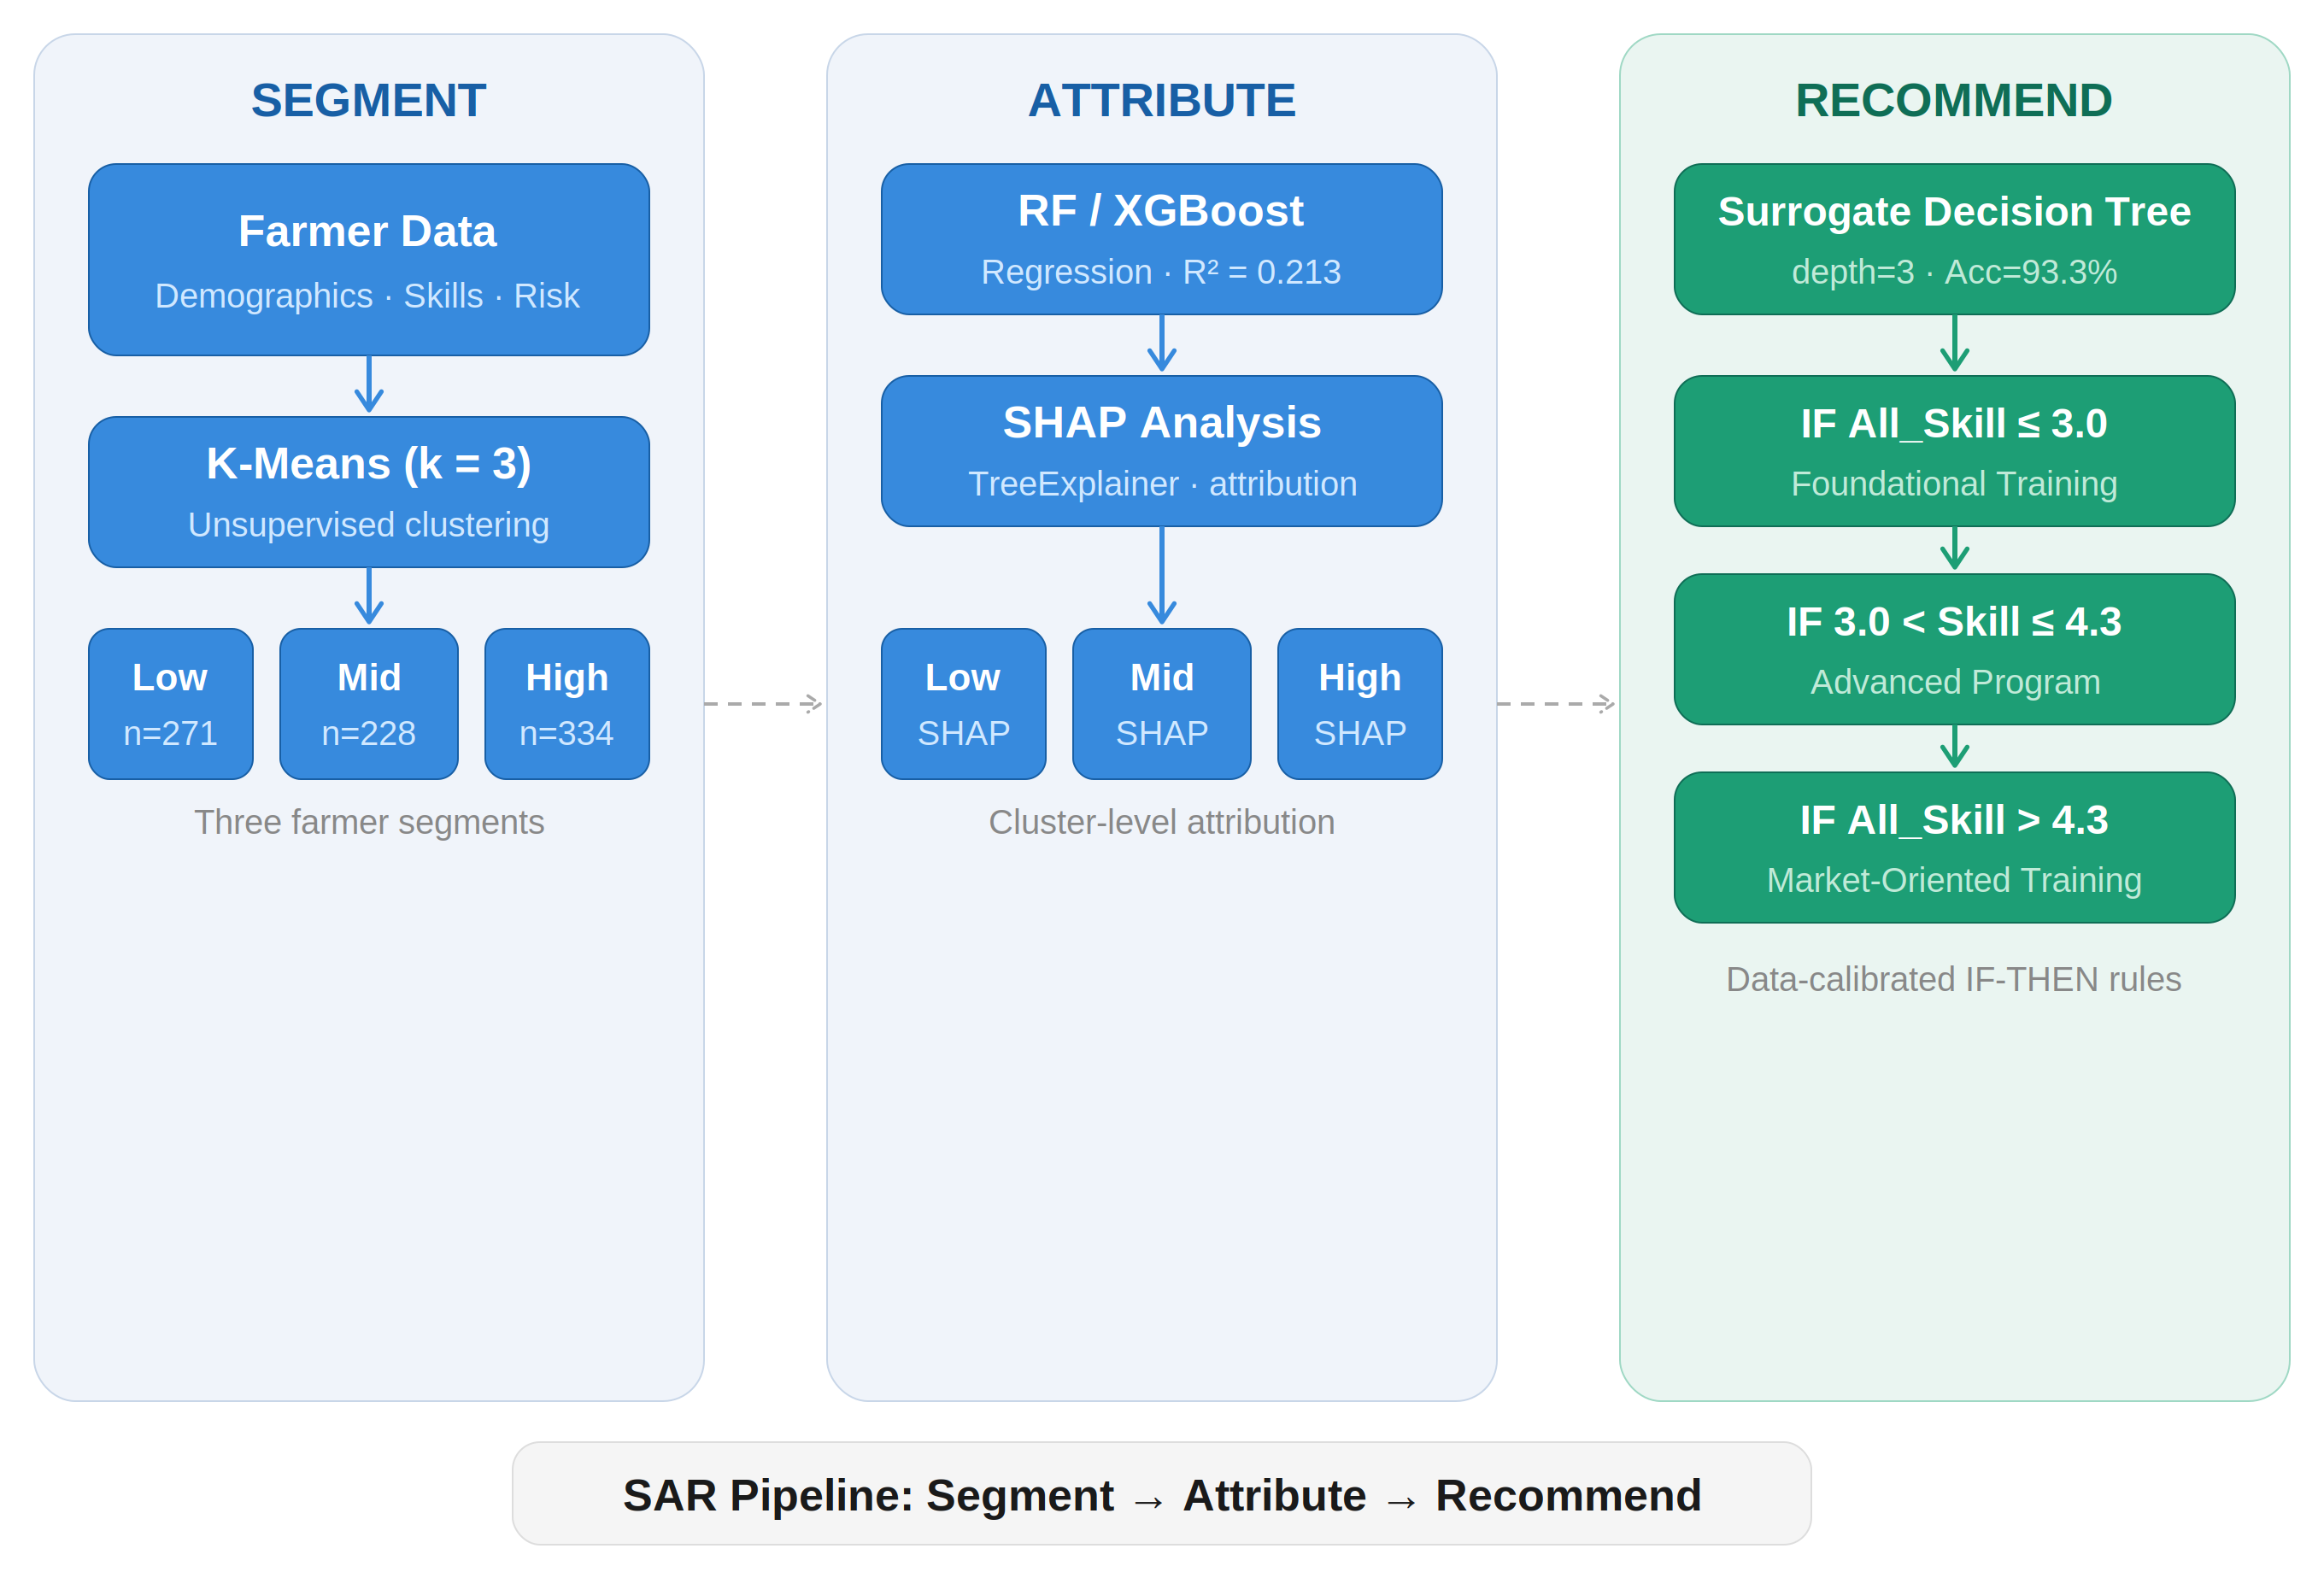
\includegraphics[width=\textwidth]{figures/fig1_framework.png}
\caption{SAR framework: three-stage pipeline (Segment, Attribute, Recommend) for interpretable allocation.}
\label{fig:framework}
\end{figure*}

\begin{figure}[htbp]
\centering

\includegraphics[width=\columnwidth]{figures/fig_elbow_silhouette.png}
\caption{Cluster validity across $k = 2$--$8$: Elbow, Silhouette, Calinski--Harabasz, and Davies--Bouldin. At $k = 3$: Silhouette $= 0.185$, CH $= 202.67$, DB $= 1.835$.}
\label{fig:elbow}
\end{figure}

\begin{figure}[htbp]
\centering

\includegraphics[width=\columnwidth]{figures/fig2_clusters_new.png}
\caption{Population segmentation via K-Means ($k = 3$) in PCA space. Three clusters show different profiles.}
\label{fig:clusters}
\end{figure}

\begin{figure}[htbp]
\centering
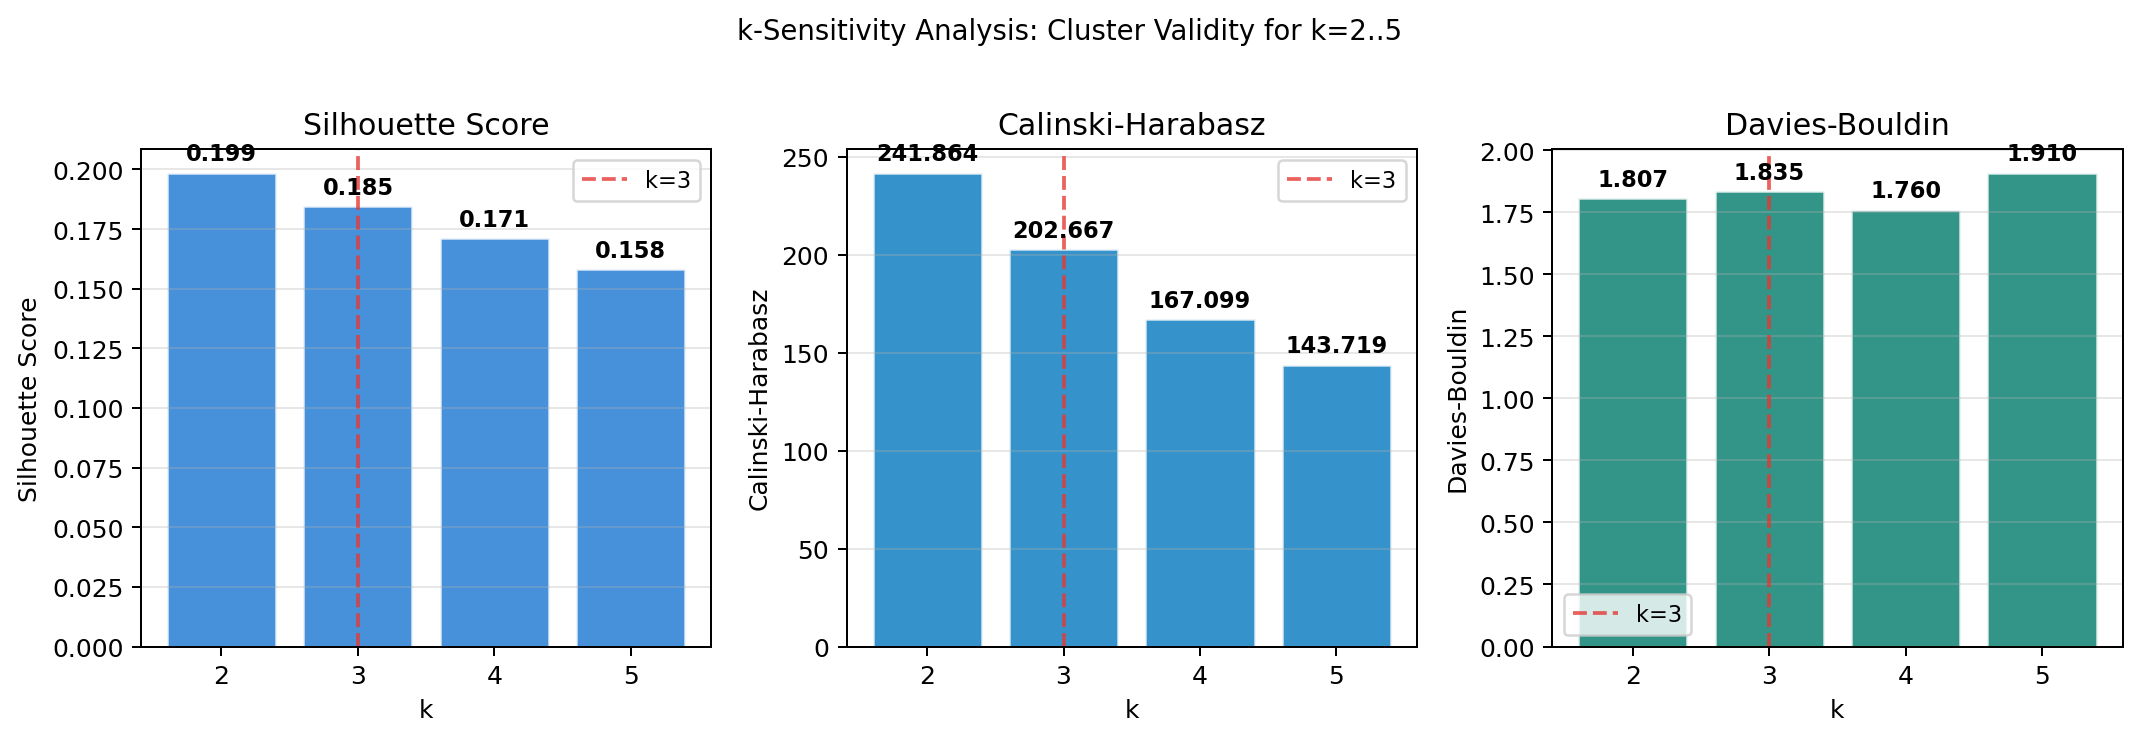
\includegraphics[width=\columnwidth]{figures/fig_k_sensitivity.png}
\caption{K-sensitivity analysis: validity indices for $k = 2$--$5$. The segment structure remains consistent across values of $k$, supporting the robustness of the three-segment solution.}
\label{fig:sensitivity}
\end{figure}

\begin{figure}[htbp]
\centering
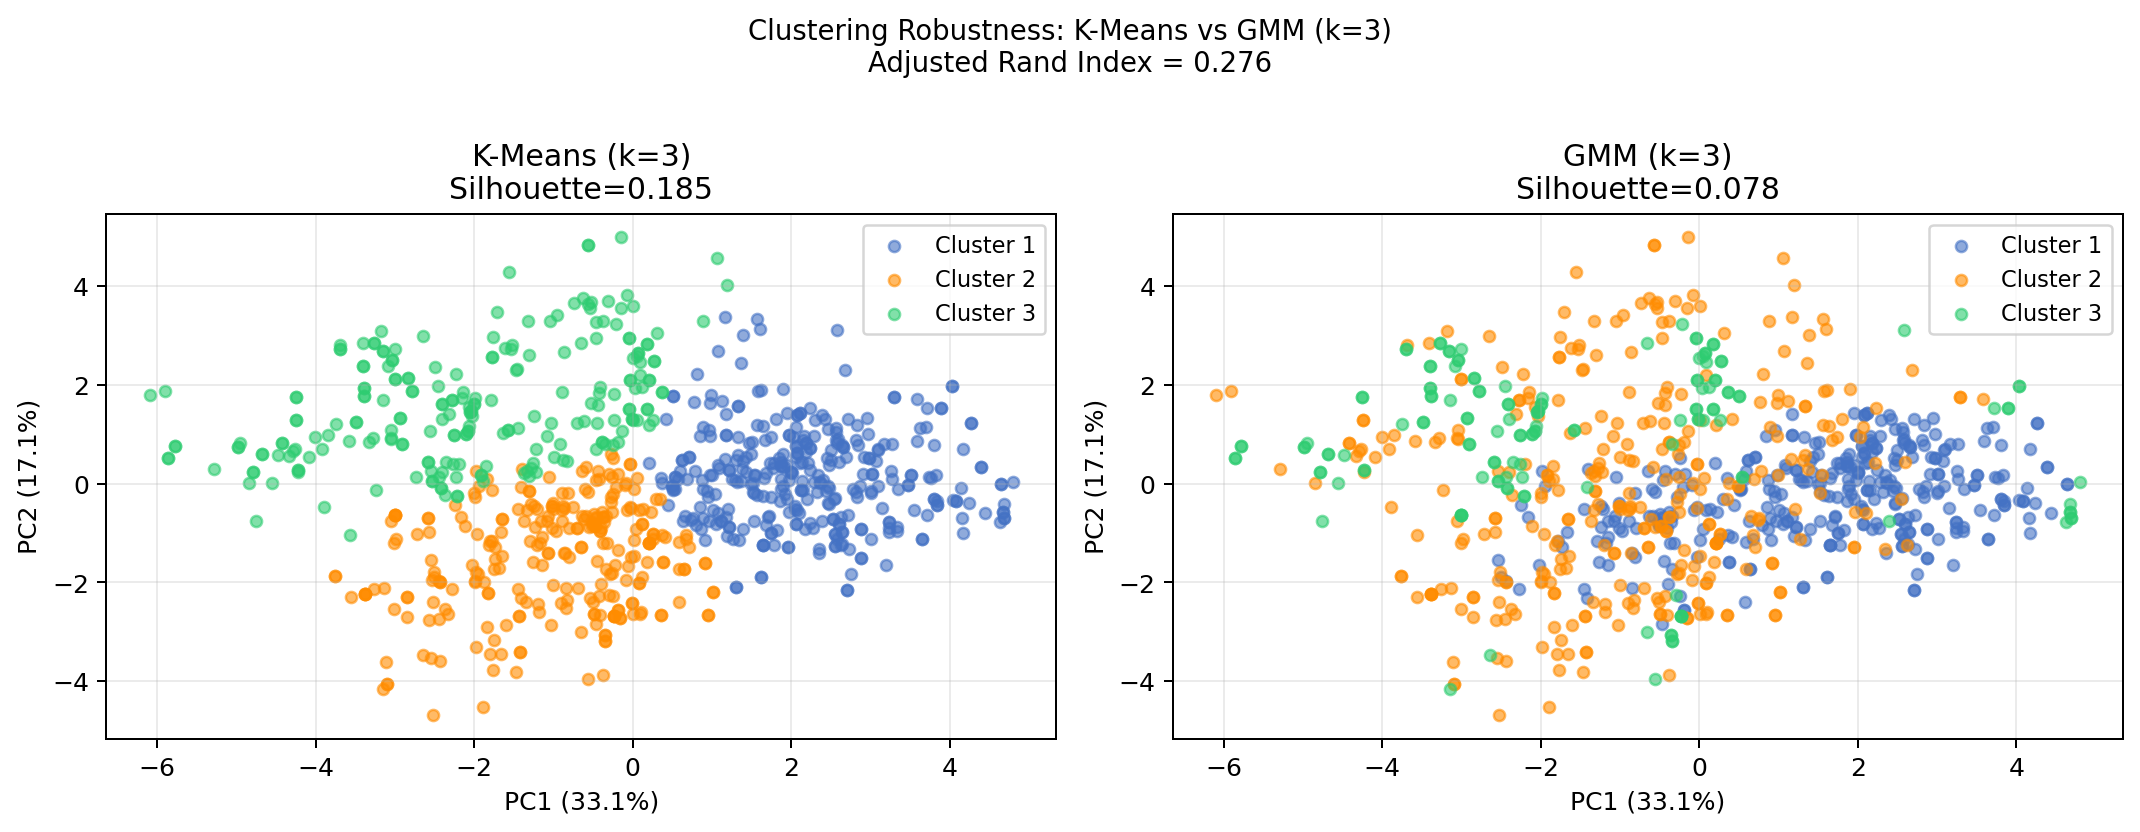
\includegraphics[width=\columnwidth]{figures/fig_gmm_robustness.png}
\caption{Clustering robustness: K-Means versus GMM ($k = 3$). Adjusted Rand Index = 0.28. K-Means produces more balanced and interpretable segment groupings than GMM in this Likert-scale dataset.}
\label{fig:gmm}
\end{figure}

\begin{figure}[htbp]
\centering

\includegraphics[width=\columnwidth]{figures/fig3_importance_new.png}
\caption{Global SHAP importance across all observations ($n = 833$). \texttt{All\_Skill} is the top driver.}
\label{fig:importance}
\end{figure}

\begin{figure}[htbp]
\centering
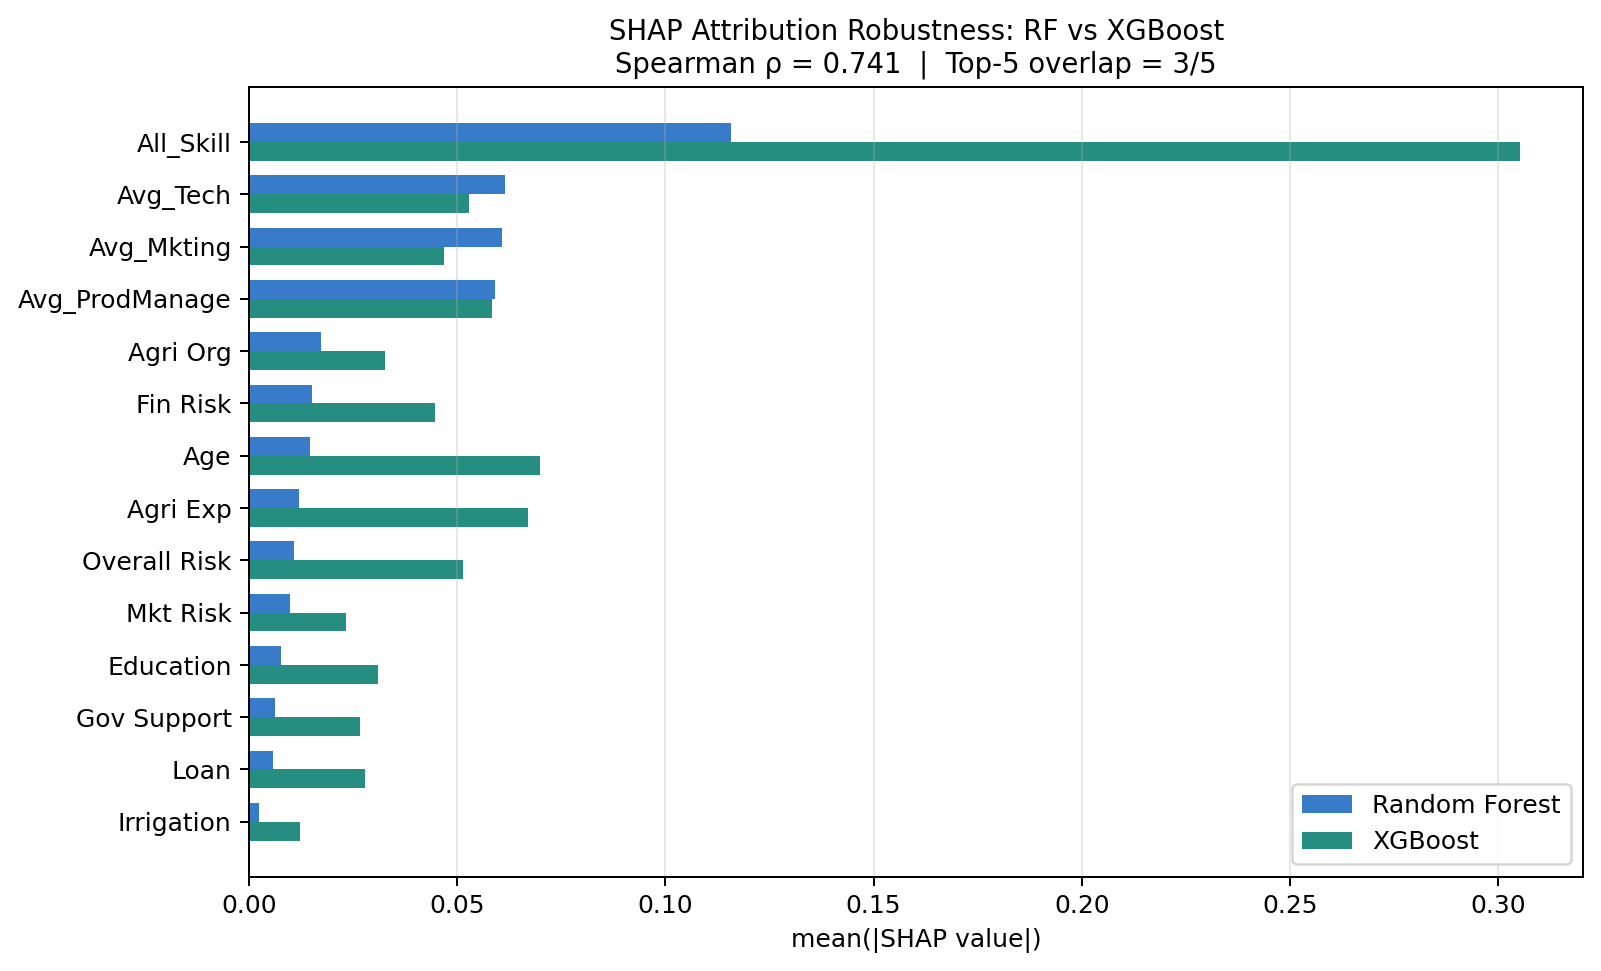
\includegraphics[width=\columnwidth]{figures/fig_shap_robustness.png}
\caption{SHAP robustness: RF vs. XGBoost ranking agreement ($\rho = 0.793$, $p < 0.001$).}
\label{fig:robustness}
\end{figure}

\begin{figure}[htbp]
\centering

\includegraphics[width=\columnwidth]{figures/fig4_shap_new.png}
\caption{SHAP beeswarm: feature contribution patterns ($n = 833$). Red = high, blue = low values.}
\label{fig:shap}
\end{figure}

\begin{figure*}[htbp]
\centering

\includegraphics[width=\textwidth]{figures/fig4b_cluster_shap_new.png}
\caption{Cluster-stratified SHAP: three segments show different feature patterns ($n = 271, 228, 334$).}
\label{fig:clusterShap}
\end{figure*}

\begin{figure*}[htbp]
\centering

\includegraphics[width=\textwidth]{figures/fig5_rules_new.png}
\caption{Surrogate decision tree (depth 3): in-sample accuracy 93.3\% ($n = 817$), held-out 91.4\%. Node labels show the splitting feature, threshold, sample count, and class distribution.}
\label{fig:rules}
\end{figure*}

%%─────────────────────────────────────────────────────────────────────────────
\section{Discussion}
%%─────────────────────────────────────────────────────────────────────────────

\subsection{Predictive Performance}

The Random Forest achieved $R^{2} = 0.283$ under farmer-level 
cross-validation, slightly better than both linear and ridge 
regression ($R^{2} = 0.257$). A modest $R^{2}$ is expected in 
studies of human learning, where skill change also depends on 
factors like motivation and trainer quality that are hard to 
measure \citep{davis2012}.

Within SAR, the Random Forest is not meant to make precise 
predictions — its main role is to generate reliable SHAP values. 
As \citet{lundberg2020} show, SHAP values can still be useful 
even when overall accuracy is moderate, as long as the model 
picks up real patterns in the data. The strong agreement between 
Random Forest and XGBoost SHAP rankings ($\rho = 0.793$, 
Fig.~\ref{fig:robustness}) confirms this. In short, the model 
is used to find patterns, not to make precise predictions.

\subsection{Refining XAI for Practical Policy}

Most XAI tools produce charts and graphs that are hard for 
non-technical staff to use in the field \citep{speith2022}. SAR 
takes a different approach — instead of presenting raw data 
visuals, it turns model findings into simple IF--THEN rules that 
extension officers can follow without any machine learning 
knowledge. This makes the system both transparent and easy to 
audit, which is important for public-sector programs 
\citep{hassija2024}.

\subsection{Segment-Specific Drivers}

The SHAP results show that different farmer groups are held back 
by different things. For Low-skill farmers, weak production 
management skills and low education are the main barriers. For 
High-skill farmers, marketing knowledge is what separates those 
who improve from those who do not. This shows that a single 
training program cannot work well for all farmers — each group 
needs a different approach.

The slight skill decline in the Low- and Moderate-skill groups 
($-0.233$ and $-0.105$) is likely due to two reasons. First, 
regression-to-the-mean: farmers who scored lowest at the start 
are more likely to show downward variation on a second assessment 
\citep{davis2012}. Second, Low-skill farmers had much lower 
participation in the Smart Farmer program (28.8\% vs 69.8\% 
for High-skill farmers), meaning many may have received little 
or no training at all \citep{anderson2004}.

\subsection{Practical Application}

SAR can be used as a simple rule-based tool for extension officers. 
This workflow follows the SAR structure illustrated in Fig.~\ref{fig:framework}. 
A typical process includes four steps:
\begin{enumerate}
  \item Record the farmer's background information (age, 
  education, skills, and resources)
  \item Assign the farmer to one of three groups using 
  the K-Means model
  \item Apply the decision rules for that group
  \item Give the farmer a specific training recommendation
\end{enumerate}

The held-out accuracy of 91.4\% confirms that the rules work 
well on new farmers. Because the rules are written in plain 
IF--THEN format, anyone can see exactly how each recommendation 
was made — no technical background needed. This is important 
for public programs that must be transparent and accountable 
to their target populations.

\subsection{Limitations}

This study has several limitations. First, all findings show 
associations between variables — they do not prove that any 
variable causes skill change. A controlled experiment would be 
needed to establish causality. Second, the farmer segments and 
rule thresholds were built using data from Thailand's Smart 
Farmer program. Using SAR in a different country or program 
would require rebuilding the model with local data. Third, the 
Silhouette scores are modest, meaning the three groups overlap 
somewhat and should be treated as practical working categories 
rather than sharply distinct types. Fourth, real-world testing 
in actual extension programs is still needed before full 
deployment. Finally, following \citet{rudin2019}, the decision 
tree rules are an approximation of the Random Forest — they 
capture the main patterns but do not reproduce every detail.

%%─────────────────────────────────────────────────────────────────────────────
\section{Conclusion}
%%─────────────────────────────────────────────────────────────────────────────

This study presents SAR, a three-stage decision support system 
for allocating agricultural training programs more effectively, 
tested on data from $n = 833$ farmers in Thailand's Smart Farmer 
initiative.

SAR combines farmer segmentation, predictive modelling, and 
explainable AI into a single pipeline that takes farmer data as 
input and produces clear training recommendations as output. The 
results show that starting skill level is the strongest predictor 
of training success, but the factors that matter second and third 
differ across farmer groups. Checking SHAP results against 
XGBoost ($\rho = 0.793$) confirms that these findings reflect 
real patterns in the data, not just features of one particular 
model.

The main contribution of this study is showing how to turn 
segment-level SHAP results into simple IF--THEN rules that 
extension officers can use directly. These rules performed 
consistently across all three evaluation methods — in-sample 
(93.3\%), held-out (91.4\%), and cross-validated 
(95.3\% $\pm$ 2.5\%) — confirming they work well on farmers 
not seen during training.

Rather than aiming for the highest possible prediction accuracy, 
SAR is designed to be transparent, consistent, and practical to 
deploy. It offers a concrete step toward bringing explainable AI 
into real agricultural extension systems.

Future work should focus on three areas: (i) testing the rules 
in other agricultural programs and countries, (ii) using 
controlled experiments to measure whether the recommended 
training actually improves farmer skills, and (iii) connecting 
SAR to live data systems so recommendations can be updated as 
new data come in \citep{yang2025,zhang2026}.

%%─────────────────────────────────────────────────────────────────────────────
\section*{Acknowledgements}
This study was supported by the United States Agency for International Development (USAID) through the Department of Agricultural and Resource Economics, Faculty of Economics at Kasetsart University, in partnership with Michigan State University. The authors are deeply grateful to all survey respondents for their cooperation. We would like to thank Professor Mywish Maredia (Michigan State University) for her invaluable guidance and the officers of the Farmer Development Division at the Department of Agricultural Extension for their assistance in facilitating data access and providing program information. 

Additionally, this work was supported by the Research and Development Institute at Bansomdejchaopraya Rajabhat University under an internal research grant program dedicated to supporting faculty members in their pursuit of academic rank advancement.

\section*{Funding}
This research was supported by the United States Agency for International Development (USAID) through Michigan State University. Additional financial support was provided by the Research and Development Institute at Bansomdejchaopraya Rajabhat University under an internal research grant program for academic rank advancement.

\section*{Ethics Statement}
This study was reviewed and exempted by the Kasetsart University Research Ethics Committee (Approval No. COE67/044, issued on 8 May 2024). All procedures were performed in accordance with the ethical guidelines for human research.

\section*{Data and Code Availability}
The anonymised dataset used in this study is available upon reasonable request, subject to the existing data-sharing agreement with the Department of Agricultural Extension, Thailand. The complete SAR framework pipeline—including clustering, Random Forest training, SHAP attribution analysis, and surrogate rule extraction scripts—is maintained in a version-controlled repository. This repository will be made publicly available on GitHub upon acceptance of this manuscript to ensure full reproducibility of our results.

\section*{Declaration of Competing Interest}
The authors declare no competing interests.

\section*{Author Contributions}
\textbf{Kitti Chiewchan:} Conceptualisation, Methodology, Machine Learning Analysis, System Architecture Design, Writing -- Original Draft, Review \& Editing. \\
\textbf{Jumtip Seneerattanaprayul:} Questionnaire Design, Data Collection, Impact Evaluation (Difference-in-Difference analysis), Result Validation.

\section*{Declaration of Generative AI and AI-assisted technologies}
During the preparation of this manuscript, the authors used Generative AI models to assist with language refinement and structural formatting. All analytical decisions, algorithmic implementations, and substantive content were developed by the authors. The authors reviewed, edited, and verified all generated material and take full responsibility for the final content of the article.

\bibliography{sample}

\end{document}